\documentclass[11pt,aspectratio=43]{beamer}
\usepackage[utf8]{inputenc}
\usepackage{amsmath, amsfonts, amssymb, amsthm}
\usepackage[T1]{fontenc}
\usepackage{lmodern}
\usepackage{xcolor}
\usepackage{setspace}
\usepackage{booktabs}
\usepackage{multirow}
\usepackage{graphicx}
\usepackage{tikz}
% \usetikzlibrary{decorations}
\usetikzlibrary{decorations.pathreplacing}
\usepackage{ulem}
\usepackage{hyperref}
\usepackage{booktabs}
\usepackage{babel}
\usepackage{makecell}
\usepackage[para,online,flushleft]{threeparttable}
\usepackage{pdfpages}
\usepackage{tcolorbox}
\usepackage{bm}
\usepackage{appendixnumberbeamer}
\usepackage{natbib}
\usepackage{caption}
\captionsetup[figure]{labelformat=empty}% redefines the caption setup of the figures environment in the beamer class.
\usetheme[compress]{Boadilla}
\usecolortheme{default}
\useoutertheme{miniframes}
\usefonttheme[onlymath]{serif}

\newcommand{\jump}[2]{\hyperlink{#1}{\beamerbutton{#2}}}
\newcommand{\orange}[1]{\textcolor{orange}{#1}}
\newcommand{\red}[1]{\textcolor{red}{#1}}

\setbeamertemplate{itemize item}{\raisebox{0.1em}{\scalebox{0.7}{$\blacksquare$}}}
\setbeamertemplate{itemize subitem}[circle]
\setbeamertemplate{itemize subsubitem}{--}
\setbeamercolor{itemize item}{fg=black}
\setbeamercolor{itemize subitem}{fg=black}
\setbeamercolor{itemize subsubitem}{fg=black}
\setbeamercolor{item projected}{bg=darkgray,fg=white}
\definecolor{blue}{rgb}{0.2, 0.2, 0.7}
\setbeamercolor{alerted text}{fg=blue}
\setbeamertemplate{enumerate items}[circle]


\setbeamertemplate{headline}{}

%==========================================
\let\olditemize=\itemize
\let\endolditemize=\enditemize
\renewenvironment{itemize}{\olditemize \itemsep1em}{\endolditemize}
\let\oldenumerate=\enumerate
\let\endoldenumerate=\endenumerate
\renewenvironment{enumerate}{\oldenumerate \itemsep1em}{ \endoldenumerate}

\DeclareMathOperator*{\argmax}{\arg\!\max}
\DeclareMathOperator*{\E}{\mathbb{E}}
\DeclareMathOperator*{\var}{\rm Var}
\DeclareMathOperator*{\cov}{\rm Cov}

\theoremstyle{definition}
\newtheorem{assume}{Assumption}
\newtheorem{lem}{Lemma}
\newtheorem{proposition}{Proposition}
\newtheorem{thm}{Theorem}
\newtheorem{corol}{Corollary}

\begin{document}
    \title[Lecture 17]{Lecture 17 \\ The Real Business Cycle Model \\ Part 4: Formal Examples}
    \author[Hui-Jun Chen]{Hui-Jun Chen}
    \institute[OSU]{The Ohio State University}
    % \date{\today}
    \date[\today]{\today \\ Credit: Kyle Dempsey}
    \setbeamertemplate{navigation symbols}{}
    \setstretch{1.2}

%-------------------------------------------------------
{
%	\usebackgroundtemplate{\includegraphics[width=1\paperwidth]{../EveningSky_cropped_edit43_bright.jpg}}
    \begin{frame}
% \vspace{3em}
        \centering
%		{\footnotesize 	ECON 4002 Intermediate Macroeconomic Theory}
        \maketitle
% \vspace{-1.5em}
% \centering
% \includegraphics[width=0.55\linewidth]{Pictures/houses.jpeg}


    \end{frame}
}

% -------------------------------------------
\setbeamertemplate{headline}
{
\setbeamercolor{section in head/foot}{fg=black, bg=white}
\vskip1em \tiny \insertsectionnavigationhorizontal{1\paperwidth}{\hspace{0.50\paperwidth}}{}
}
%------------------------------------------


\begin{frame}{Overview}
\label{slide:Overview}
    \begin{itemize}
        \item Recall that in Lecture 13, there is no production in dynamic model.
        \item The following $ 5 $ lectures is for \textbf{Real Business Cycle} (RBC) model:
        \begin{itemize}
            \item Lecture 14: consumer
            \item Lecture 15: firm
            \item Lecture 16: competitive equilibrium
            \item Lecture 17: formal example
            \item Lecture 18: application to bring RBC to data
        \end{itemize}
    \end{itemize}
\end{frame}

\section{Model Analysis}
\label{sec:Model_Analysis}

\begin{frame}{Assumptions}
\label{slide:Assumptions}
    \begin{itemize}
        \item \textbf{consumer}: assume discounting factor $ \beta \in ( 0, 1 ) $ and utility function is
        \begin{center}
            $ \displaystyle \tilde{U}( C, N, C') = \ln C + \beta \ln C' + \gamma \ln ( 1-N ),$
        \end{center}
        where $ \gamma > 0 $, and consumer endowed with $ 1 $ unit of time.
        \begin{itemize}
            \item we assume no dis-utility in date 1 labor supply to simplify analysis
        \end{itemize}
        \item \textbf{firm}: assume production is Cobb-Douglas in both periods:
        \begin{center}
            $ \displaystyle Y = z K^{\alpha} N^{1-\alpha} $ and $ \displaystyle Y' = z' K'^{\alpha} N'^{1-\alpha} $,
        \end{center}
        where $ K $ is initial capital, TFP $ z = 1 $, and depreciation $ \delta \in ( 0, 1 ) $
        \item \textbf{government}: spend $ G $ and $ G' $, which is financed by lump-sum taxes $ T, T' $ and deficit $ B $
    \end{itemize}
\end{frame}

\begin{frame}{Competitive Equilibrium}
\label{slide:Competitive_Equilibrium}
    \scriptsize
    Given exogenous quantities $ \{ G, G', z, z', K \} $, a competitive equilibrium is a set of (1) consumer choices $ \{ C, C', N_{S}, N'_{S}, l, l', S \} $; (2) firm choices $ \{ Y, Y', \pi, \pi', N_{D}, N'_{D}, I, K' \} $; (3) government choices $ \{ T, T', B \} $, and (4) prices $ \{ w, w', r \} $ such that
    \begin{enumerate}
        \item Taken $ \{ w, w', r, \pi, \pi' \} $ as given, consumer chooses $ \{ C', N_{S}, N'_{S} \} $ to solve
            %
            \begin{center}
                $
                \displaystyle
                \max_{C', N_{S}, N'_{S}} \ln \left(
                    w N_{S} + \pi - T +
                    \frac{w' N'_{S} + \pi' - T' - C'}{1+r}
                \right) + \beta \ln C' + \gamma \ln ( 1-N_{S} )
                $,
            \end{center}
            where we can back out $ \{ C, S, l, l' \} $.
        \item Taken $ \{ w, w', r \} $ as given, firm chooses $ \{ N_{D}, N'_{D}, K' \} $ to solve
            %
            \begin{center}
                $
                \displaystyle
                \max_{N_{D}, N'_{D}, K'} z K^{\alpha} N_{D}^{1-\alpha} - w N_{D} - [ K' - ( 1-\delta ) K ] + \frac{z' ( K' )^{\alpha}( N'_{D} )^{1-\alpha} - w' N'_{D} + ( 1-\delta ) K'}{1+r}
                $,
            \end{center}
            where we can back out $ \{ Y, Y', \pi, \pi', I \} $.
        \item Taxes and deficit satisfy $ \displaystyle T + \frac{T'}{1+r} = G + \frac{G'}{1+r} $ and $ G - T = B $.
        \item All markets clear: (i) labor, $ N_{S} = N_{D} $ \& $ N'_{S} = N'_{D} $; (ii) goods, $ Y = C + G $ \& $Y' = C' + G' $; (iii) bonds at date 0, $ S = B $.
    \end{enumerate}
\end{frame}

\begin{frame}{Step 0: Result Implied by Assumptions}
\label{slide:Step_0__Result_Implied_by_Assumptions}
    \begin{enumerate}
        \item $ N'_{S} = 1 $, since consumer don't value leisure at date 1.
        \begin{itemize}
            \item If consumer don't value leisure, then choose the highest possible $ N'_{S} $ can expand the budget set without decreasing the utility.
        \end{itemize}
        \item $ N'_{D} = N'_{S} = 1 $, by future labor market clearing.
        \item The future wage $ w' $ is determined by $ MPN' $:
        %
        \begin{equation*}
            MPN' = z ( 1-\alpha ) \left(
                \frac{K'}{N'_{D}}
            \right)^{\alpha}
        ,\end{equation*}
        %
        where $ N'_{D} = 1 $ leads to
        %
        \begin{equation*}
            w' = z ( 1-\alpha ) ( K' )^{\alpha}
        .\end{equation*}
        %
    \end{enumerate}
\end{frame}

\begin{frame}{Step 1: Firm's Current Labor Demand}
\label{slide:Step_1__Firm_s_Current_Labor_Demand}
    \begin{columns}
        \begin{column}{0.5\textwidth}
            \begin{figure}
                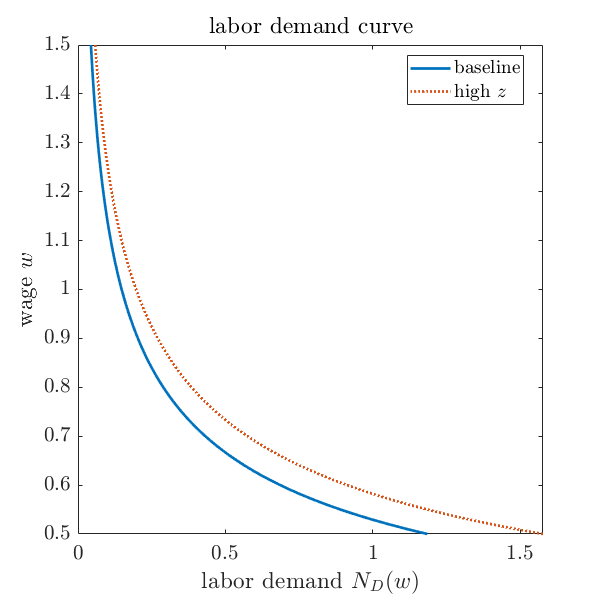
\includegraphics[width=\textwidth]{./figures/LaborDemandTFP.png}
            \end{figure}
        \end{column}
        \begin{column}{0.5\textwidth}
            For date 0 labor demand,
            %
            \begin{align*}
                MPN
                    & = z ( 1-\alpha ) \left(
                        \frac{K}{ N_{D}}
                    \right)^{\alpha} = w
                \\
                \Rightarrow N_{D}
                    & = \left(
                        \frac{z ( 1-\alpha )}{w}
                    \right)^{\frac{1}{\alpha}} K
            \end{align*}
            %
            \begin{itemize}
                \item $ N_{D} \downarrow $ in current wage $ w $
                \item $ N_{D} \uparrow  $ in current TFP $ z $ (dotted line)
                \item $ N_{D} $ invariant to interest rate
            \end{itemize}
        \end{column}
    \end{columns}
\end{frame}

\begin{frame}{Step 2: Consumer \& Current Labor Supply}
\label{slide:Step_2__Consumer_Analysis}
    \begin{itemize}
        \item \alert{labor supply} at date 0:
        %
        \begin{align*}
           MRS_{l, C}
                & = -MRS_{N, C} = -\frac{D_{N} \tilde{U}( \cdot )}{D_{C} \tilde{U}( \cdot )}
            \\
                & = -\frac{-\gamma/( 1-N_{S} )}{1/C} = \frac{\gamma C}{1-N_{S}} = w
        \end{align*}
        %
        \item \alert{Saving} at date 0:
        %
        \begin{equation*}
            MRS_{C, C'} = \frac{1/C}{b/C'} = \frac{C'}{bC} = 1+r
        \end{equation*}
        %
        \item Recall $ N'_{S} = 1$, we can denote the $ x $ notation to be the part of the income that is NOT \alert{directly affected by consumer choice}:
        %
        \begin{equation*}
            x = \pi - T \quad \text{and} \quad x' = w' + \pi' - T'
        \end{equation*}
        %
    \end{itemize}
\end{frame}

\begin{frame}{Step 2: Consumer \& Current Labor Supply (Cont.)}
\label{slide:Step_2__Consumer_Analysis_for_Current_Labor_Supply__Cont__}

\end{frame}
<++>





\section{Appendix}
\label{sec:Appendix}

\appendix
% -------------------------------------------
\setbeamertemplate{headline}
{
\setbeamercolor{section in head/foot}{fg=black, bg=white}
\vskip1em \tiny \insertsectionnavigationhorizontal{1\paperwidth}{\hspace{0.50\paperwidth}}{}
}
%------------------------------------------
\begin{frame}\frametitle{}
\begin{columns}
\label{Appendix}
\column{1\linewidth}
\centering
{\Large \alert{Appendix}}
\end{columns}
\end{frame}
%------------------------------------------
\begin{frame}[allowframebreaks]{References}
\footnotesize
\bibliographystyle{$BIB_STYLE}
\bibliography{$BIBFILE}
\end{frame}

\end{document}


